\documentclass{report}

\input{~/latex/template/preamble.tex}
\input{~/latex/template/macros.tex}

\title{\Huge{Chapter 3 Notes}}
\author{\huge{Matt Warner}}
\date{\huge{}}
\pagestyle{fancy}
\fancyhf{}
\rhead{Math 211 - Calculus For Business \& Social Science}
\lhead{\leftmark}
\cfoot{\thepage}
% \usepackage[default]{sourcecodepro} \usepackage[T1]{fontenc}

\pgfpagesdeclarelayout{boxed}
{
  \edef\pgfpageoptionborder{0pt}
}
{
  \pgfpagesphysicalpageoptions
  {%
    logical pages=1,%
  }
  \pgfpageslogicalpageoptions{1}
  {
    border code=\pgfsetlinewidth{1.5pt}\pgfstroke,%
    border shrink=\pgfpageoptionborder,%
    resized width=.95\pgfphysicalwidth,%
    resized height=.95\pgfphysicalheight,%
    center=\pgfpoint{.5\pgfphysicalwidth}{.5\pgfphysicalheight}%
  }%
}

\pgfpagesuselayout{boxed}

\begin{document}
  \maketitle
  \section*{3.1 - Using First Derivaties to Classify Maximum and Minimum Values}
  \bigbreak \noindent \bigbreak \noindent
  \hrule
  \bigbreak \noindent
  \vspace{-3mm}\subsection*{Increasing and Decreasing Functions}
  \bigbreak \noindent
  If the graph of a function rises from left to right over an interval $I$, the function is said to be increasing on, or over, $I$.
  \bigbreak \noindent
  If the graph drops from left to right, the function is said to be decreasing on, or over, $I$.
  \begin{figure}[ht]
  \centering
  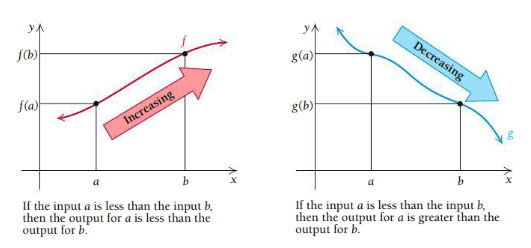
\includegraphics[width=0.65\textwidth]{  /home/mattw/niu/Math211/latexdocs/figures/paste.png}
  \end{figure}
\bigbreak \noindent
We can define these concepts as follows.
\begin{mdframed}
  \vspace{2mm}

  A function $f$ is \textbf{increasing} over $I$ if, for every $a$ and $b$ in $I$, 
  $$ \text{if } a < b, \ \ \ \text{then } f(a) < f(b)$$
  A function $f$ is \textbf{decreasing} over $I$ if, for every $a$ and $b$ in $I$,
  $$ \text{if } a < b, \ \ \ \text{then } f(a) > f(b)$$
\end{mdframed}
\bigbreak \noindent
The above definitions can be restated in terms of slopes of secant lines
\end{document}
